% Chapter 2

\chapter{Background} % Main chapter title

\label{Chapter2} % For referencing the chapter elsewhere, use \ref{Chapter1} 

\lhead{Chapter 2. \emph{Background}} % This is for the header on each page - perhaps a shortened title

%----------------------------------------------------------------------------------------
  Chapter 2 explains the required background knowledge to understand the topic of the thesis. This chapter includes four sections, which is about MapReduce, Hadoop, MapReduce versions and cloud computing. 
   
    The Authors in Google implemented many special-purpose computation paradigms in the past years. The purpose of these special-purpose computations were to process large amount of raw data such as crawled web documents, web requests, logs, etc. The process of large data helps Google to compute various graph of derived data, such as inverted indices, various graph representation of web documents, summaries of number of pages crawled per host, the set of most frequent queries in a data , etc.\cite{mapreduce}\\

In a paper published in 2004, MapReduce was introduced by Google \cite{mapreduce}. MapReduce is used to process large datasets and data for applications and problems like image analysis, graph-based problems, machine learning algorithms \cite{mahout}.

%----------------------------------------------------------------------------------------


  
  
\section{MapReduce}

MapReduce is a programming model and associated implementation to process large datasets in parallel.  The approach used in MapReduce is that, for each query the entire dataset or great portion of it, is processed. MapReduce is batch query process which has the ability to run single query against whole dataset. The power is that, using MapReduce approach reasonable response time is provided for queries. Programs written in MapReduce style are automatically parallelized and executed over set of distributed machines, which allow programmers to easily utilize resources of distributed systems. \\

 The MapReduce program reads input key/value pairs and generates output key and value pairs. A MapReduce program consist of map and reduce phases, where both map and reduce phases are defined as map and reduce functions written by programmers. The map function reads input data as  key/value pairs and generates intermediate values. The output of map function is processed by MapReduce platform to the reduce function, which reads intermediate data and merges all values associated with the same intermediate key. MapReduce is designed to run jobs that lasts minutes or hours on dedicated hardware in a single data center, with very high bandwidth interconnects.\cite{tom3}\\

 MapReduce is some how restrictive programming model, where users are limited to key and value types. Both key and value are related in pre-specified ways, and the mappers pass keys and values to reducers for further process. The reducer(s) sorts the received data and write it to output file.      

For better understanding, an example of MapReduce logical data flow is explained in figure \ref{fig:map-reduce}. The goal of MapReduce in below example is to process weather dataset and find maximum global temperature recorded for each year. The map function reads the data and emits the year and recorded temperature for the year as key and value pairs. It is good to drop bad records such as missing temperatures, suspects and erroneous in map phase. The output of map function is not directly injected to reduce function, it is processed by MapReduce framework to sort them by key (in this case year is the key for MapReduce). As result, each year appears with list of temperatures, the reducer finds the maximum temperature for each year and store it in output file.  
  
%\begin{verbatim}
\begin{figure}[htbp]
  \centering
    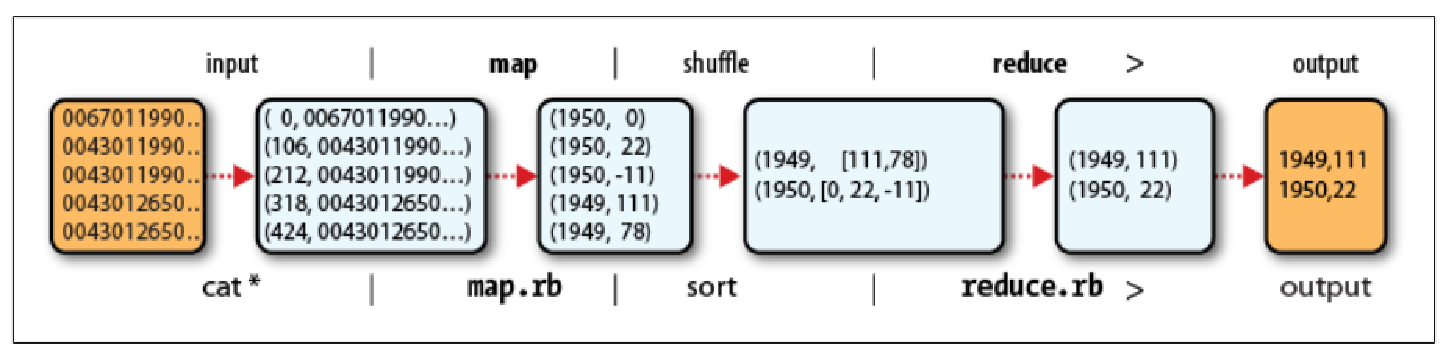
\includegraphics[width=\textwidth,height=\textheight,keepaspectratio]{./Figures/map-reduce.pdf}
    \rule{35em}{0.5pt}
  \caption{MapReduce logical data flow \cite{tom3}}
  \label{fig:map-reduce}
\end{figure}
%\end{verbatim}


\section{Hadoop}
% Lalith - The name Hadoop is not an acronym; it is made-up name by kid of Doug Cutting calling his yellow elephant toy “Hadoop”

Hadoop is an open source implementation of MapReduce programming model used to process huge datasets. Hadoop was created by Doug Cutting, the creator of Apache Lucene, the widely used text search library\cite{tom3}. Hadoop processes huge datasets in a key/value pattern search. Where key is the data to be searched and value is the result of search for specific key. \\

 Usually, the datasets to be processed by Hadoop is large enough and in term of TeraBytes. Hadoop splits large datasets into small fixed size chunks of data, called "jobs". For further process, Hadoop splits jobs into smaller work-units called "tasks", a single job may consist one or many tasks. Using Hadoop scheduler, tasks are scheduled for process and execution on datanodes machines in a Hadoop cluster. \\
 
 Though, Hadoop can run on a single machine, but as it is used to process huge datasets, a set of machines forming Hadoop cluster is used to process data. The machines in Hadoop cluster works in master-slave pattern. The master machine is called "Namenode" and slaves are called "Datanodes". To store and retrieve the data, Hadoop uses different filesystem than normal filesystems, which is called Hadoop Distributed File System (HDFS). HDFS has bigger size of data blocks than normal filesystems of operating system. \\
 
There are two versions of MapReduce deployed in Hadoop, called MapReduce version 1(classic MapReduce) and MapReduce version 2( Yarn). The data process on each MapReduce version is processed using different components and techniques. \\

 Before explaining the detail of how does Hadoop works, here are some terms that helps the understanding of Hadoop/MapReduce data process: \\

\textbf{Job} MapReduce job is unit of work that needs to be processed by set of computers (also referred as computational resources in this thesis), in this case Hadoop cluster. It consist of input data ( raw data to be processed), job configuration information and MapReduce program. 

\textbf{Task}‌ To run the jobs, Hadoop divides it into smaller units, called tasks. Tasks are real data that is processed in the system. There are two types of tasks: map tasks and reduce tasks. Both, map and reduce tasks are predefined user functions, that is used to process data. For example, a map task reads the input data and searches for key in that data. The result of map tasks are directed to reducer tasks/function, to sort and write the output values. 

\textbf{Job Size} The job size is configurable, depending on job type and requirement the size of job may change to bigger or smaller size. If the job size is very small, then the job creation and map creation time will dominant the over all execution time of jobs. Having many small jobs mean that the execution time for each job is smaller comparing to large input. Running small jobs in parallel on Hadoop cluster, the total time of processing all small jobs will be smaller than total time to process large input dataset. The default job size is 64 MB (which is programmable to change), which is equal to HDFS block size. Such job size is good for Rack Locality Feature of Hadoop.\\ 


\subsection{HDFS}


 HDFS is the filesystem of Hadoop which stores large datasets across cluster of computers in reliable and distributed manner. HDFS is designed to stream data in high bandwidth to user applications.
“HDFS is a filesystem designed for storing very large files with streaming data access patterns, running on clusters of commodity hardware” \cite{tom3}. According to \cite{tom3} HDFS‌ is designed to accommodate the follow:

\textbf{Very Large Files } The “very large” in this context refers to files in size of hundreds of gigabytes or terabytes.

\textbf{Streaming Data} The efficient data processing idea behind HDFS design was based on write once and read many times. Typically, dataset is generated or copied from source and process/query is executed on large portion, if not all, of dataset. Therefore, the time to read the whole file is more important than reading the first record. 
  
%\subsection{Common \LaTeX{} Math Symbols}
\textbf{Commodity Computers } HDFS does not require expensive highly-available and reliable hardware. It is designed to run over cluster of commodity hardware (commonly available hardware from multiple vendors) where the  failure chances of hardware is very high. HDFS‌ is robust to hardware failure, it is designed to continue process and work without noticing the user application from hardware failure. As the idea behind HDFS design is for large data files and the read time for the whole file is more important, thus HDFS will not work so well for low latency applications and small files. \\
 
 Not for each and every data and application HDFS‌ is fair data storage and retrieve method. Below are examples of cases where HDFS‌ may not work well for applications that fall into below categories. \  

\textbf{Low-latency Data Access } As the idea behind HDFS was for data with high throughput, loading large files, where total load time of a large file is critical, applications that require low latency in tens of milliseconds, will not work well using HDFS.
 
\textbf{Lots of Small Data } The information about stored and processed by Hadoop data files are stored as inode data. The inode data and list of blocks belonging to each file is called metadata. The namenode stores the filesystem metadata in Random Access Memory (RAM). The number of files in namenode is limited by memory size. Each file, directory, and block takes 150 bytes in memory, it is feasible to have millions of files, but billions is beyond the capacity of available RAM and can not be supported.
   
\subsubsection{HDFS Blocks}
 
The minimum amount of data or sequence of bytes (or bits) that disk can read or write is called disk block size which is typically 530 Bytes. To read and write data into blocks, filesystem blocks which are in size of kilo bytes are created on top of disk blocks. Generally, the disk blocks are transparent to filesystem.\cite{tom3} HDFS also has the concept of block; it's default block size is 64 megabytes. The size of HDFS block can be modified to larger sizes for example 128 megabytes or 512 megabytes. HDFS breaks large files into fixed size chunks called HDFS blocks. Each block is stored independently across multiple datanodes of Hadoop cluster. For small file chunks, full capacity of HDFS is not occupied by HDFS. \\

 The time to read and write on disk depends on two factors: seek time and data transfer rate of the disk. The time needed to move HEAD (data reader or write component of disk) to the block from where it should read or write is called seek time. The amount of data that disk can read and transfer in a second is called disk transfer rate which is usually calculated as megabytes per second. HDFS blocks are larger in comparison to disk block size, this is to reduce the seek time of the disk. For large blocks, the data transfer time is significantly bigger compared to seek time to move to beginning of the block, thus time to transfer multiple files is equal to disk transfer rate.\\

  An advantage of the block structure is that if a file is larger than available capacity of single disk in the one of the machines in Hadoop cluster, it can be stored across multiple disks on the datanodes of Hadoop cluster. Which makes it unnecessary that all blocks of the file should be stored on same single disk. 

%----------------------------------------------------------------------------------------


\subsection{Namenode and Datanode}

 As explained in \cite{tom3}, HDFS cluster consist of two types of nodes (machines) which operates in master-worker pattern: single namenode (the master) and number of datanodes (workers). The total number of datanodes and namenode forms an HDFS cluster. The namenode is responsible to store and manage filesystem namespace and the metadata for all files and directories in the tree. The information is stored in local disk in two different files "namespace image" and "edit log".\\

  Datanodes are workers that stores and retrieves data when they are told by namenode. The datanodes updates the namenode with list of data blocks that they are storing. All nodes in a Hadoop cluster communicate with each other using TCP-based protocols(TCP-based RPC‌ framework). To ensure reliability of data, multiple copies of data are stored across multiple datanodes. By default, three copies of the data is stored across multiple datanodes in a Hadoop cluster.\\
   

All the information about filesystem is stored on namenode. The namenode knows all the datanodes on which the blocks for a given file is located. In case, if namenode data is erased (due to failure or any other reason), then, all the files on filesystem is lost because there is no way of how to reconstruct data blocks. Therefore, having resilient namenode to failure becomes important for which Hadoop provides two mechanisms.
 

 The first mechanism is to configure Hadoop in a way that it write the steady state of the namenode to multiple filesystems as backup copy. The writes are atomic operations that can write to local disk and to a remote Network File System (NFS) mounted disk space.


 The second solution is to run another namenode as secondary namenode and merge the image-space image with edit logs in order to prevent edit log files from becoming too large. Since secondary namenode requires as much CPU and memory as namenode (primary namenode), usually, it runs on separate physical machine. The secondary namenode keeps copy of the merged namespace image, and this copy can be used in case of namenode failure. Usually, when namenode fails copy of namenode data which are on NFS is copied to secondary namenode and secondary namenode becomes the new primary namenode.


   


%----- Data -----
%Hadoop stores meta-data and application data separately. The Meta data is stored in server machine so called Name Node. The user %application data is stored on other servers so called Data Node(s).  The advantage of this strategy is that data transfer is %multiplied and there are more chances to locate computation near the data (Data Locality)\cite{sailfish}.


\subsection{Schedulers}

Hadoop uses scheduling algorithm to assign jobs/tasks to datanodes for execution. The default Hadoop scheduler had First In First Out (FIFO) mechanism for submitted jobs. The jobs were managed in a queue structure,  and the first submitted jobs were scheduled first for execution on the cluster. After completion of first job, the second job, and so on, jobs are executed on Hadoop cluster. The scheduler is one of the key factors on the performance of Hadoop, thus, literature suggested optimization to Hadoop scheduler. The performance and side effects of optimized Hadoop scheduler like Capacity Share Scheduler, Fairshare Scheduler and Speculative Task Execution are analysed in this thesis.  



 



%----------------------------------------------------------------------------------------

%\section{Hadoop Schedulers}

\section{MapReduce Versions}

There are multiple features added time by time to MapReduce, which created multiple versions of MapReduce. In this section we explain the two versions of MapReduce. To coordinate and manage the process and execution of jobs, few more components are used by Hadoop. The component used in Hadoop depends on Hadoop versions. Up to now, Hadoop takes advantage of two versions of MapReduce, called MapReduce version 1, and MapReduce version 2(YARN). Both versions have different components and methodology to process the jobs. 

\subsubsection{MapReduce Version 1} 
MapReduce Version 1, which is also called classic MapReduce has the following methodology to run jobs (brief):

  - Client is the one that submits jobs to MapReduce to be processed. 
  - The JobTracker is the component used to coordinate the jobs for process. 
  - The TaskTracker is the component to run the tasks (tasks are small splits of jobs).
  - A scheduler is used to schedule the tasks for process.
  - HDFS‌ is used to store and retrieve the data.  
 
The figure \ref{mrv1}  explains the structure of MapReduce version 1. 

\begin{figure}[htbp]
  \centering
    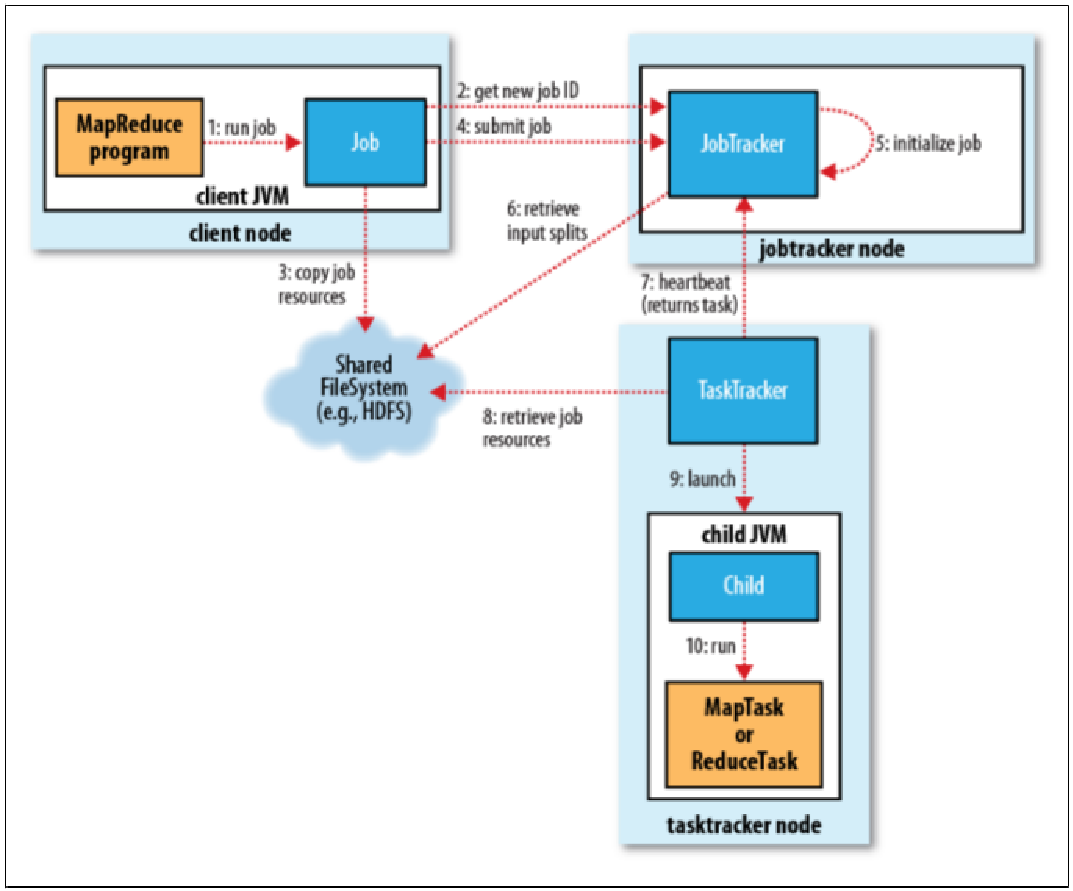
\includegraphics[width=10 cm,height=10 cm]{./Figures/mrv1.pdf}
    \rule{28em}{0.5pt}
  \caption{MapReduce Version 1 Architecture \cite{tom3}}
  \label{mrv1}
\end{figure}
 


Detail:
Usually the data to be process by Hadoop is very large dataset. Hadoop divides this large dataset input to small fixed-size "input split” or “split”. Each split is called MapReduce job. The splits are fed as input to user defined map function. Map functions read each record of input split and process it.\\

Job execution are controlled by two components of Hadoop called JobTracker and TaskTracker. JobTracker is responsible to run all jobs on system. It coordinates job execution by scheduling tasks on tasktracker. The JobTracker maintains records about status of each job and monitors the progress of each task. The TaskTracker executes tasks on nodes and sends progress report to JobTracker. In case if a task execution failed, the JobTracker is the one which reschedules the task on same or different TaskTracker.\\




















\subsubsection{MapReduce version 2 (Yarn)}

For clusters with more than 4,000 nodes, MapReduce version 1, had scalability bottlenecks. To overcome this issue , the new version of MapReduce called Yet Another Resource Negotiator (YARN) was developed by Yahoo!‌ in 2010 \cite{tom3}.\\  

 To overcome the shortcoming of MapReduce version 1, YARN splits the functions of JobTracker into two separate components. JobTracker is responsible for job scheduling and task progress monitoring, YARN‌ uses application manager and resource manager as two separate daemons for these functions. \\

\begin{figure}[htbp]
  \centering
    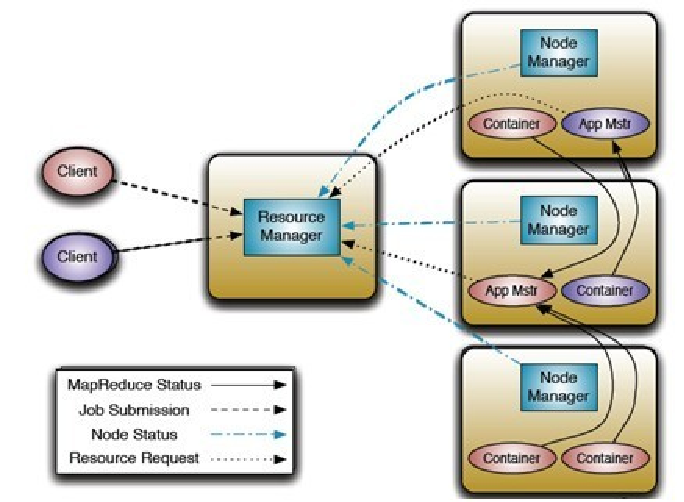
\includegraphics[width=10 cm,height=10 cm]{./Figures/yarn.pdf}
    \rule{25em}{0.5pt}
  \caption{YARN‌ architecture \cite{yarn}}
  \label{yarn}
\end{figure}

As illustrated in figure \ref{yarn}, there is single resource manager and per-application applications-master. Application could be single job or group of jobs. The per-application master, negotiates for resources with resource manager and works with node manager to monitor tasks. There is an agent per datanode (worker machine) called node manager, that  monitors the resource usage for application running on datanode, and submits the status report of each node to resource manager.\\
 
Resource manager is responsible to manage resource usage across Hadoop cluster. It has two main components:

The Scheduler which is responsible to allocate resources to applications and does not perform the monitoring or tracking status of the application. The scheduler performs resources provision based on resource requirements of applications. The abstract notion \i{Container} is used for resource, where resource could be incorporate of elements like memory, CPU, disk, network, etc. The scheduler has plug-in policy, based which resources can be be configured and shared among different applications for example capacity and fairshare schedulers.\\

The application-manager is the entity that accepts the submitted jobs, negotiates for the container to execute per-application application-master and in case of failure, restarts the application-master. The application-master is responsible to negotiate required resource container for application (job or jobs) from scheduler, track and monitor the progress of the application. The application-master is created per application and runs for the duration of its application, and finishes after complete process of the application.\\  


YARN‌ is compatible with MapReduce version 1, all jobs of MapReduce version 1 just needs recompilation to be executed on YARN \cite{yarn}.   



  




\section{Cloud Computing}

 Cloud Computing is a distributed computing paradigm that enables the provision of available, scalable and reliable on-demand resources over a network, primarily the Internet connection \cite{nist}. Applications, networks, platforms, storage, processing power, service, etc can be resources in cloud computing. Resources can be provisioned and released with minimal management interaction of the provider. The composition of resources , mostly as virtualized pool of resources are provisioned to customer and can be released with minimal management interaction of provider or customer. Since, clients are unaware of how and where are the resources, the term "cloud" which is an abstraction paradigm used for such services. 

\subsection{Service Models}
  The classification of cloud computing paradigm according to the level of abstraction and control provided to them, offers several types of services. A well known classification of cloud services, adopted by United States National Institute of Standards and Technology (NIST)‌, is explained below: 


\textbf{Software as a Service (SaaS)} SaaS model provides the facility to consumer to use software applications running in cloud infrastructure. To access the services, user interface through which user can access the services from any device using applications such as web browser. The infrastructure on which service is running, is owned and managed either by provider or third party and consumer has limited or no control over underlying resources. Examples of SaaS providers are: Google Docs, Dropbox and GitHub. \\  


\textbf{Platform as a Service (PaaS)} PaaS model allows the consumers to create, use and deploy 
applications on the cloud provider's infrastructure. Consumers can use programming languages and tools supported by provider to create and deploy applications. The control level given to consumer is
 more than SaaS, but limited to control over deployed applications and configuration 
settings of applications hosting environment. Examples of PaaS providers are: Google App Engine, Microsoft Azure.\\    



\textbf{Infrastructure as a Service (IaaS)} IaaS provides the capability to the consumer to use fundamental computing resources such as processing, storage, networks. The consumer is also able to deploy arbitrary software including operating system on the cloud. The consumer has control over software, operating systems and deployed applications, but the physical infrastructure that runs the services is owned by provider. Typically, the physical resources are shared among multiple users or organizations by virtualization hyper-visor. Examples of IaaS‌ providers are: RackSpace and Amazon EC2\\ 


\subsection{Deployment Models}

The classification of cloud computing can be done based on deployment models. NIST \cite{nist} defined the following four categories as deployment model for cloud computing:

\textbf{Public Cloud} 
The cloud is made available to general public or groups of people and industries. The infrastructure is either owned by cloud provider or third party. 
  
\textbf{Private Cloud} 
The cloud is operated exclusively by single organization. The cloud maybe managed and owned by other organization or third party. 
 
\textbf{Community Cloud} 
The Cloud is shared by several organizations that have common interests such as share mission , security or university campus. It maybe owned and managed by organization forming community or a third party. 


\textbf{Hybrid Cloud} 
The composition of two or more clouds deployments by standardized technology to single cloud infrastructure , that provides portability is called hybrid cloud. \

















